\documentclass[10pt]{article}
\usepackage[a4paper,margin=0.85in]{geometry}
\usepackage[T1]{fontenc}
\usepackage{lmodern}
\usepackage{microtype}
\usepackage{amsmath,amssymb}
\usepackage{booktabs,tabularx,multirow}
\usepackage{graphicx}
\usepackage{xcolor}
\usepackage{caption}
\usepackage{subcaption}
\usepackage{enumitem}
\usepackage{array}
\usepackage[section]{placeins}   % keep floats inside their section
\newcolumntype{Y}{>{\raggedright\arraybackslash}X}
\newcolumntype{P}[1]{>{\raggedright\arraybackslash}p{#1}}
\renewcommand{\arraystretch}{1.12}
\usepackage[colorlinks=true,linkcolor=blue!50!black,urlcolor=blue!50!black,citecolor=blue!50!black]{hyperref}
\captionsetup{font=small,labelfont=bf}
\setlist{nosep,leftmargin=*}
\setlength{\parskip}{3pt}
\setlength{\parindent}{0pt}

% \res{...} marks numbers that come from the Kaggle judge; filled after judging.
\newcommand{\res}[1]{\textcolor{red}{#1}}
\newcommand{\pend}{\res{--}}
% Judge results are generated by scripts/fill_report_results.py into results_auto.tex / auto_interpretation.tex.
\IfFileExists{results_auto.tex}{% generated by scripts/fill_report_results.py -- do not edit by hand
\newcommand{\JudgeModel}{\texttt{google/gemini-3.6-flash}}
\newcommand{\ResUFwin}{52.2\% (95\% CI 48\%--57\%)}
\newcommand{\ResHHwin}{69.0\% (95\% CI 64\%--73\%)}
\newcommand{\RowUFA}{95 & 123 & 82 & 31.7\% & 53.7\% & 52.2\% (48\%--57\%) & 0/0 & 61\%}
\newcommand{\RowHHthreeH}{171 & 72 & 57 & 57.0\% & 75.0\% & 69.0\% (64\%--73\%) & 0/0 & 76\%}
\newcommand{\RowHHoneH}{135 & 121 & 44 & 45.0\% & 75.4\% & 65.2\% (61\%--69\%) & 0/0 & 65\%}
\newcommand{\RowHHtenH}{111 & 60 & 129 & 37.0\% & 46.2\% & 47.0\% (42\%--52\%) & 0/0 & 80\%}
\newcommand{\RowHHthreeA}{73 & 129 & 98 & 24.3\% & 42.7\% & 45.8\% (42\%--50\%) & 0/0 & 61\%}
\newcommand{\RowUFH}{75 & 145 & 80 & 25.0\% & 48.4\% & 49.2\% (45\%--53\%) & 0/0 & 61\%}
\newcommand{\RowSFTA}{199 & 63 & 38 & 66.3\% & 84.0\% & 76.8\% (73\%--81\%) & 0/0 & 79\%}
\newcommand{\RowLoraA}{4 & 36 & 0 & 7 & 19 & 14}
\newcommand{\RowLoraB}{28 & 12 & 0 & 5 & 9 & 26}
\newcommand{\RowLoraC}{35 & 5 & 0 & 2 & 7 & 31}
}{}
\providecommand{\RepoURL}{\res{\texttt{https://github.com/<user>/small-model-alignment}}}
\providecommand{\JudgeModel}{\res{\texttt{google/gemini-3.6-flash}}}
\providecommand{\ResUFwin}{\res{xx}}
\providecommand{\ResHHwin}{\res{xx}}
\providecommand{\RowUFA}{\pend & \pend & \pend & \pend & \pend & \pend & \pend & \pend}
\providecommand{\RowHHthreeH}{\pend & \pend & \pend & \pend & \pend & \pend & \pend & \pend}
\providecommand{\RowHHoneH}{\pend & \pend & \pend & \pend & \pend & \pend & \pend & \pend}
\providecommand{\RowHHtenH}{\pend & \pend & \pend & \pend & \pend & \pend & \pend & \pend}
\providecommand{\RowHHthreeA}{\pend & \pend & \pend & \pend & \pend & \pend & \pend & \pend}
\providecommand{\RowUFH}{\pend & \pend & \pend & \pend & \pend & \pend & \pend & \pend}
\providecommand{\RowSFTA}{\pend & \pend & \pend & \pend & \pend & \pend & \pend & \pend}
\providecommand{\RowLoraA}{\pend & \pend & \pend & \pend & \pend & \pend}
\providecommand{\RowLoraB}{\pend & \pend & \pend & \pend & \pend & \pend}
\providecommand{\RowLoraC}{\pend & \pend & \pend & \pend & \pend & \pend}
\newcommand{\code}[1]{\texttt{\small #1}}
\newcommand{\piw}{\log \pi_\theta(y_w\mid x)}
\newcommand{\pil}{\log \pi_\theta(y_l\mid x)}
\newcommand{\rw}{\log \pi_{\mathrm{ref}}(y_w\mid x)}
\newcommand{\rl}{\log \pi_{\mathrm{ref}}(y_l\mid x)}

\title{\vspace{-1.2cm}\textbf{Instruction Tuning and Direct Preference Optimization\\on Qwen2.5-0.5B}\\[2pt]
\large Programming Assignment 2 --- Final Report}
\author{Fazal Rehman \quad (Roll No.\ 27100294)\\ \small Repository: \RepoURL}
\date{}

\begin{document}
\maketitle
\vspace{-0.8cm}

\begin{abstract}
\noindent We post-train \code{Qwen/Qwen2.5-0.5B} with a from-scratch supervised fine-tuning (SFT) loop on 30k
UltraChat examples, then run two from-scratch DPO experiments from the same SFT checkpoint: one on 15k single-turn
HH-RLHF pairs and one on 15k UltraFeedback pairs. A third track tunes \code{SmolLM2-360M-Instruct} with TRL's
\code{DPOTrainer} and LoRA toward a Gordon-Ramsay-style persona. All models are compared on fixed prompt sets with
blinded, order-swapped pairwise judgments from \JudgeModel{} through Kaggle's model proxy.
SFT lowers held-out response NLL from 1.396 to 1.331 and makes the model stop properly (65\% of base-model answers hit the
512-token cap). UF-DPO reaches 0.775 validation reward accuracy. For HH, the guide learning rate ($10^{-6}$) barely changes
refusal behavior, so we sweep $\{1,3,10\}\times10^{-6}$ and select $3\times10^{-6}$ by validation reward accuracy (0.654). It
raises refusal and redirection on harmful prompts, while $10^{-5}$ over-optimizes into incoherent over-refusal. Judged against SFT,
UF-DPO scores \ResUFwin{} on AlpacaEval and HH-DPO scores \ResHHwin{} on the helpful/harmless set (ties counted as half).
\end{abstract}

%=====================================================================
\section{Repository, models, and data}
%=====================================================================
\textbf{Code.} The training math (batching, masking, response log-probabilities, SFT and DPO losses) lives in
\code{sma/core.py}, and \code{submission\_adapter.py} wraps it for the private grader. The loops are
\code{sma/train\_sft.py} and \code{sma/train\_dpo.py}; neither uses HF \code{Trainer} or TRL. The 7 public tests and 15 additional
edge-case tests pass (truncation that removes EOS, \code{pad\_token\_id}$=$\code{eos\_token\_id}, missing pad/EOS
tokens, row order, brute-force log-prob checks, gradient-accumulation equivalence).

\textbf{Prompt format.} The same template is used for SFT, both DPO runs, and evaluation: Qwen ChatML with the system message
``You are a helpful assistant.'' (\code{sma/prompts.py}). The response is followed by the tokenizer EOS
\code{<|endoftext|>}, and generation stops on \code{<|im\_end|>} or \code{<|endoftext|>}. Prompt and response are tokenized
separately and concatenated, EOS is appended \emph{before} truncation to 512 tokens, rows are right-padded, and all masks
are derived from true row lengths (important because Qwen's pad id equals its EOS id).

\textbf{Seeds and decontamination.} Seed 42 is used for every shuffle, the evaluation subset, data order, and A/B order. Training
prompts that exactly match (after whitespace and case normalization) an evaluation instruction are removed.

\begin{table}[!htbp]
\centering\small
\caption{Data actually used. Counts are from \code{outputs/data/data\_stats.json}.}
\label{tab:data}
\begin{tabularx}{\linewidth}{@{}l P{4.4cm} Y r@{}}
\toprule
Track & Source & Filtering & Train / val \\
\midrule
SFT & UltraChat-200k (\code{HuggingFaceH4/}\allowbreak\code{ultrachat\_200k}) & first user/assistant turn; prompt $\le$256 tok; prompt$+$response$+$EOS $\le$512 tok (30{,}000 kept of 59{,}174 scanned) & 30{,}000 / 1{,}000 \\
HH-DPO & \code{Anthropic/hh-rlhf}, harmless-base + helpful-base & single-turn only (24{,}971 of 86{,}372); chosen $\ne$ rejected; prompt $\le$256 tok; 50/50 harmless/helpful & 15{,}000 / 1{,}000 \\
UF-DPO & UltraFeedback (\code{HuggingFaceH4/}\allowbreak\code{ultrafeedback\_binarized}) & single-turn; score margin $\ge$1 (drops 18{,}447 near-ties); prompt $\le$256 tok (33{,}474 eligible) & 15{,}000 / 1{,}000 \\
LoRA-DPO & provided \code{ramsay\_style\_}\allowbreak\code{preferences.json} & seeded 90/10 split & 198 / 22 \\
\midrule
\multicolumn{4}{@{}p{\linewidth}@{}}{\textbf{Evaluation sets:} AlpacaEval subset of 300 of 805 prompts drawn with \code{random.Random(42).sample}
(\code{eval\_sets/alpaca\_eval\_300\_seed42.json}); the provided HH set (300 prompts, 10 categories $\times$ 30); our persona set of
40 prompts (10 each: cooking, coding, general help, safety-sensitive).}\\
\bottomrule
\end{tabularx}
\end{table}

%=====================================================================
\section{Experimental configuration}
%=====================================================================
For each pair $(x, y_w, y_l)$ we minimize the DPO objective, with response-only summed log-probabilities:
\begin{align}
\mathcal{L}_{\mathrm{DPO}} &= -\log\sigma\!\Big(\beta\big[(\piw-\pil)-(\rw-\rl)\big]\Big), \label{eq:dpo}\\
r_w &= \beta\big(\piw-\rw\big), \qquad r_l=\beta\big(\pil-\rl\big). \nonumber
\end{align}
Reward accuracy is $\Pr[r_w>r_l]$ (strict) and the margin is $\mathbb{E}[r_w-r_l]$. The SFT loss is the \emph{token mean} of
response NLL. With gradient accumulation it is normalized by the response-token count of the whole accumulation
window, so the accumulated gradient equals the gradient of the token mean over the full effective batch.

\begin{table}[!htbp]
\centering\small
\caption{Values used for the submitted checkpoints (one H100 80GB on Modal; seed 42 throughout).}
\label{tab:config}
\begin{tabularx}{\linewidth}{@{}P{2.6cm} Y Y Y Y@{}}
\toprule
 & SFT & HH-DPO & UF-DPO & LoRA-DPO \\
\midrule
Model & Qwen2.5-0.5B & SFT best & SFT best & SmolLM2-360M-Instruct \\
Trainable & full (494M) & full & full & LoRA $r{=}16$, $\alpha{=}32$, drop.\ 0.05; q,k,v,o,gate,up,down (8.68M, 2.34\%) \\
Optimizer & AdamW (0.9, 0.999) & AdamW & AdamW & AdamW (TRL) \\
Peak LR, schedule & $2\!\times\!10^{-5}$, cosine, 3\% warmup & $3\!\times\!10^{-6}$ constant (sweep $\{1,3,10\}\!\times\!10^{-6}$) & $10^{-6}$ constant & sweep $\{5\!\times\!10^{-5}, 10^{-4}, 2\!\times\!10^{-4}\}$, cosine, 10\% warmup \\
Weight decay / clip & 0.1 (not on norms/emb.) / 1.0 & 0 / 1.0 & 0 / 1.0 & 0 / 1.0 \\
Micro $\times$ accum $=$ eff. & $16\times2=32$ & $4\times8=32$ pairs & $4\times8=32$ pairs & $4\times2=8$ \\
Precision & bf16 autocast, FP32 weights & same & same & bf16 \\
Max len / prompt & 512 / 256 & 512 / 256 & 512 / 256 & 512 / 256 \\
Epochs (steps) & 1 (938) & 1 (469) & 1 (469) & 3 (75) / 3 (75) / 5 (125) \\
$\beta$, reference & --- & 0.1, frozen \code{sft/best} & 0.1, frozen \code{sft/best} & 0.1, adapter disabled \\
Selection & min val loss (step 900) & max val reward acc (step 400) & max val reward acc (step 400) & final adapter; run chosen by judge (\S\ref{sec:lora}) \\
Wall-clock & 6.0 min & 7.3 min (each run) & 12.4 min & $\sim$1 min \\
\bottomrule
\end{tabularx}
\end{table}

\textbf{Decoding (identical within every comparison).} Greedy (\code{do\_sample=False}, so temperature and top-$p$ are
unused), \code{max\_new\_tokens}$=$512, \code{repetition\_penalty}$=$1.1, no $n$-gram blocking, bf16, left-padded
batches. The Qwen models use the ChatML template above; the SmolLM2 models use their own chat template.
\textbf{Judge.} \JudgeModel{} at temperature 0, 5 pairs per request, $\ge$5\,s between attempts,
$\le$3 retries, both A/B orders.

%=====================================================================
\section{Parameter choices and deviations}
%=====================================================================
\begin{table}[!htbp]
\centering\small
\caption{Deviations from the guide. R = resource-driven, P = performance-driven, D = design or measurement choice.}
\label{tab:dev}
\begin{tabularx}{\linewidth}{@{}P{2.4cm} P{2.5cm} P{2.6cm} c Y@{}}
\toprule
Item & Guide & Ours & Type & Reason and observed effect \\
\midrule
Hardware & T4$\times$2, fp16+scaler & H100, bf16 & R & bf16 has fp32 range, so no loss scaling is needed and no steps are skipped; FP32 master weights unchanged. The fp16 path is kept (\code{--precision fp16}). \\
SFT micro-batch & $2\times16$ & $16\times2$ & R & Same effective batch; window-level token normalization makes the gradient identical (unit-tested). \\
DPO micro-batch & $1\times32$ & $4\times8$ & R & Same 32 pairs per step; per-micro-batch means are reweighted. \\
DPO optimizer & RMSprop/AdamW & AdamW & D & RMSprop has no bias correction: its second moment starts at 0, so early steps are about $10\times$ lr without warmup. AdamW is stable at a fixed $10^{-6}$. \\
Reference model & fp16, 2nd GPU & FP32 + same autocast & D & Policy and reference are bit-identical at step 0: we measured loss $=0.6931=\log 2$ and accuracy $=0$, margin $=0$ on both tracks, so diagnostics measure learning rather than precision noise. \\
SFT length filter & --- & fit in 512 & P & Every target ends in EOS. SFT outputs: 0\% truncated on the sanity set vs.\ 65.3\% for the base model on AlpacaEval. \\
UF pair filter & --- & margin $\ge1$ & P & Removes ties and near-ties (30\% of pairs), which carry little preference signal. \\
HH-DPO LR & $10^{-6}$ & $3\!\times\!10^{-6}$ & P & At $10^{-6}$ the model still complies with 100\% of harmful/cyber/doxxing prompts (Table~\ref{tab:hhsweep}). Of $\{1,3,10\}\!\times\!10^{-6}$ we select by validation reward accuracy, not by judge results. The guide run is still reported. \\
LoRA LR / epochs & --- & 3-point sweep & P & The first run ($5\!\times\!10^{-5}$) saturated validation accuracy but barely changed greedy outputs, so we swept LR and epochs and compared runs by judged style \emph{and} quality (\S\ref{sec:lora}). \\
\bottomrule
\end{tabularx}
\end{table}

%=====================================================================
\section{Training behavior}
%=====================================================================
\begin{figure}[!htbp]
\centering
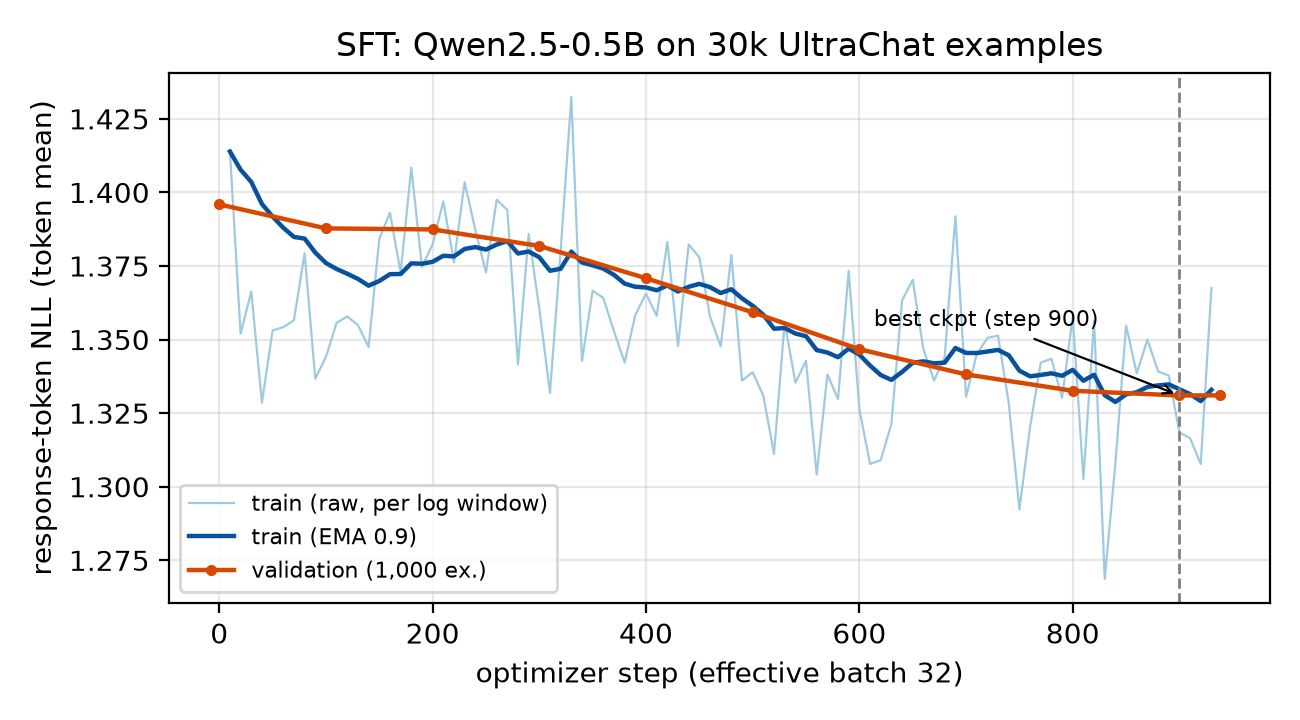
\includegraphics[width=0.62\linewidth]{figures/sft_loss.png}
\caption{SFT response-token NLL. Train loss per 10-step window (raw and EMA 0.9); validation on 1{,}000 held-out
examples every 100 steps. The dashed line marks the selected checkpoint (step 900).}
\label{fig:sft}
\end{figure}

\textbf{SFT.} Validation NLL falls monotonically from 1.396 (base) to 1.331 (step 900; step 938 is equal to 4 d.p.).
It is nearly flat at peak LR (1.388 at steps 100--200) and drops mostly during cosine decay, with no sign of overfitting.
The modest change is expected: the base model already models UltraChat-style text, and SFT mainly teaches the
turn format and when to stop.

\begin{figure}[!htbp]
\centering
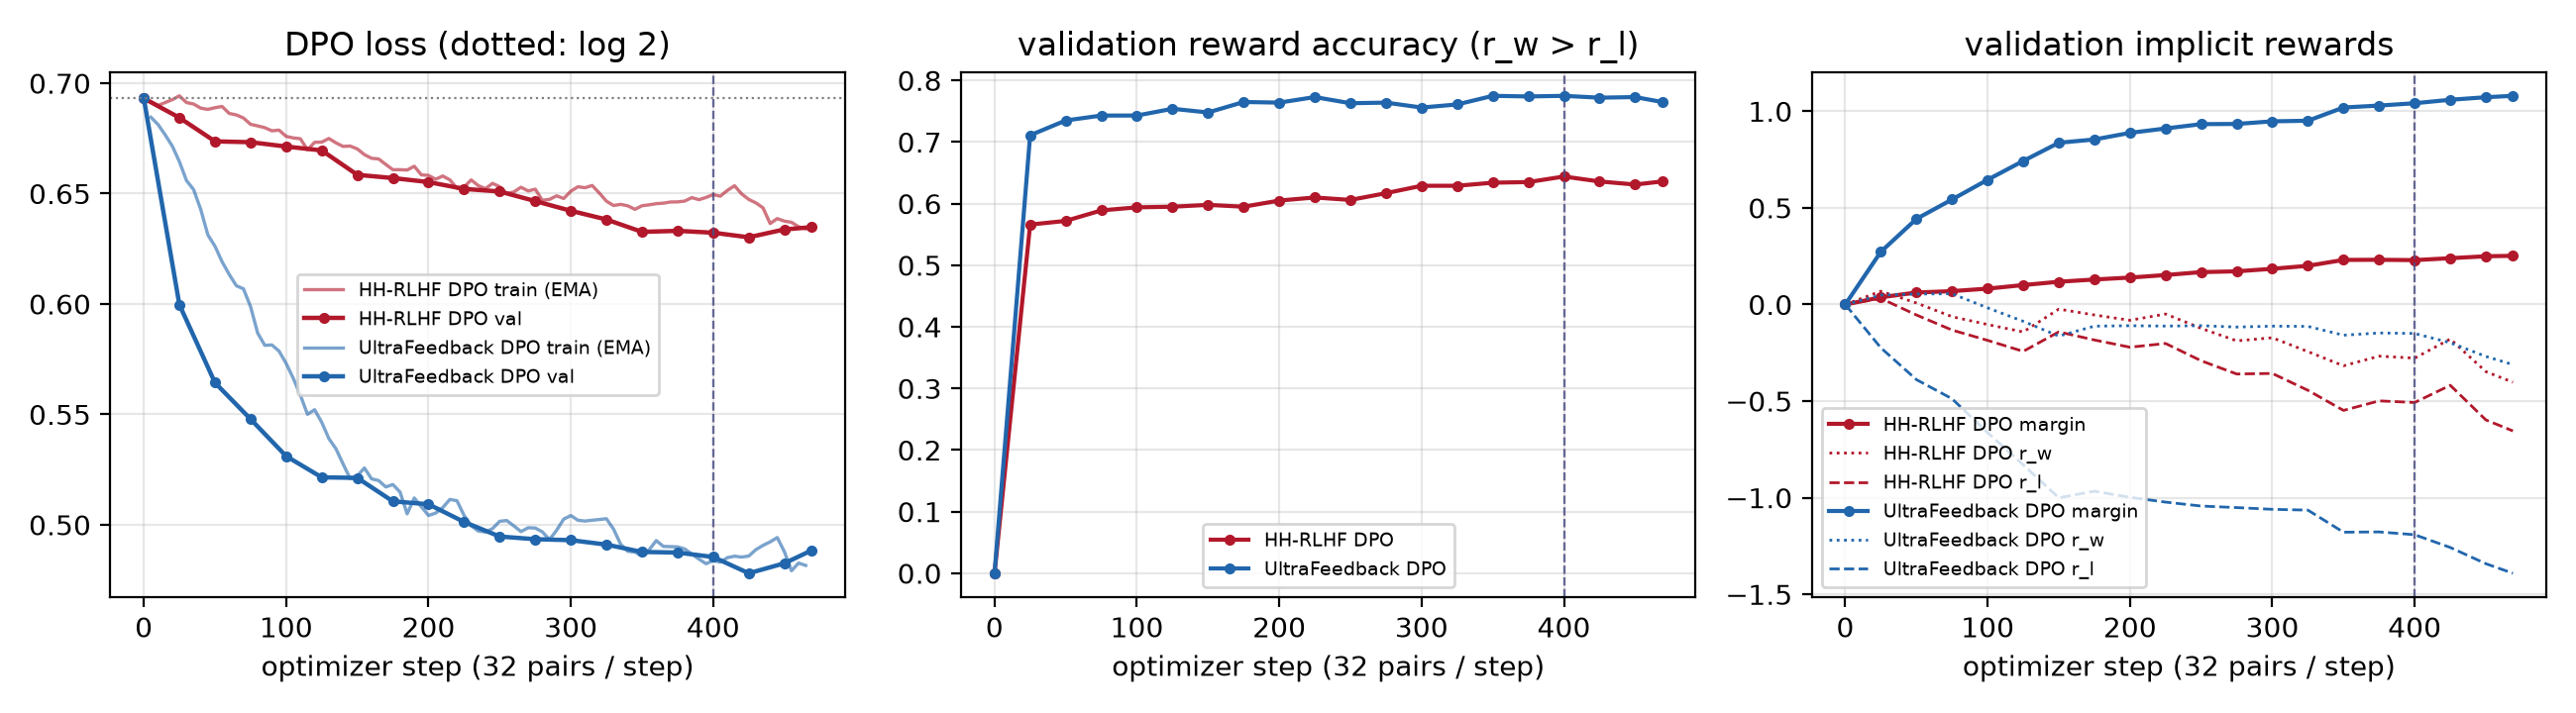
\includegraphics[width=\linewidth]{figures/dpo_curves.png}
\caption{From-scratch DPO. Left: train loss (EMA 0.9) and validation loss (dotted line: $\log 2$). Middle: validation
reward accuracy. Right: validation margin and implicit rewards $r_w$ (dotted), $r_l$ (dashed). Vertical lines mark the
selected checkpoints (step 400 for both runs). Evaluation every 25 steps on 1{,}000 pairs.}
\label{fig:dpo}
\end{figure}

\textbf{DPO.} Both runs start at exactly $\log 2$ with zero accuracy and margin (all rewards tied), as
Eq.~\ref{eq:dpo} predicts for identical policy and reference. UF learns much faster and further: accuracy 0.711 after 25 steps and
0.775 at step 400 (margin 1.04). HH reaches 0.644 (margin 0.23) and climbs slowly throughout, consistent with HH's
noisier labels. In both runs \emph{both} implicit rewards become negative, which means the chosen log-likelihood also falls:
\begin{center}\small
\begin{tabular}{@{}lccccc@{}}
\toprule
Run (best step) & val acc & margin & $r_w$ & $r_l$ & $\log\pi(y_w)$ / $\log\pi(y_l)$: init $\to$ best \\
\midrule
HH-DPO (400) & 0.644 & 0.230 & $-0.278$ & $-0.507$ & $-119.5\to-122.3$ \;/\; $-115.1\to-120.2$ \\
UF-DPO (400) & 0.775 & 1.042 & $-0.150$ & $-1.191$ & $-319.7\to-321.2$ \;/\; $-276.5\to-288.4$ \\
\bottomrule
\end{tabular}
\end{center}
DPO therefore widens the gap mainly by pushing rejected responses down (the ``likelihood displacement'' effect). Accuracy saturates after
about 350 steps in both runs, so the best-accuracy checkpoint (step 400) and the final checkpoint differ little.

\textbf{HH learning-rate sweep.} Table~\ref{tab:hhsweep} and Fig.~\ref{fig:hhsweep} show that validation accuracy is nearly flat across a
$10\times$ LR range, while the margin and the behavior change a lot. The refusal columns use a keyword heuristic (refusal, decline,
or redirection to professional help in the first 400 characters) on the 30 prompts per category of HH-eval. They are a measurement aid; the
judge results in \S\ref{sec:res} are the actual evaluation. At $10^{-5}$ the chosen log-likelihood collapses ($-119.5\to-138.4$),
validation loss rises above the other runs, and greedy outputs become long, repetitive refusals (69\% hit the token cap).
We therefore select $3\!\times\!10^{-6}$, which has the best validation accuracy \emph{and} loss.

\begin{table}[!htbp]
\centering\small
\caption{HH-DPO learning-rate sweep (one epoch, $\beta{=}0.1$, all from \code{sft/best}). Columns 2--5 are validation diagnostics at the
best step (400; 469 for $10^{-5}$); the last five columns are measured on HH-eval generations.}
\label{tab:hhsweep}
\setlength{\tabcolsep}{4pt}
\begin{tabular}{@{}l cccc c ccccc@{}}
\toprule
 & \multicolumn{4}{c}{Validation (1{,}000 pairs)} & & \multicolumn{5}{c}{HH-eval generations: refuse/redirect rate} \\
\cmidrule(lr){2-5}\cmidrule(l){7-11}
LR & acc & margin & loss & $\log\pi(y_w)$ & tokens (capped) & harmful & cyber & privacy & hate & benign \\
\midrule
SFT (reference) & --- & --- & 0.693 & $-119.5$ & 177 (0.7\%) & 0\% & 0\% & 0\% & 3\% & 0\% \\
$10^{-6}$ (guide) & 0.644 & 0.230 & 0.632 & $-122.3$ & 152 (0.7\%) & 0\% & 0\% & 0\% & 0\% & 0\% \\
$3\!\times\!10^{-6}$ (selected) & \textbf{0.654} & 0.420 & \textbf{0.631} & $-122.5$ & 137 (0.7\%) & 10\% & 3\% & 20\% & 23\% & 0\% \\
$10^{-5}$ & 0.649 & 0.723 & 0.695 & $-138.4$ & 405 (69\%) & 90\% & 100\% & 90\% & 100\% & 23\% \\
\bottomrule
\end{tabular}
\end{table}

\begin{figure}[!htbp]
\centering
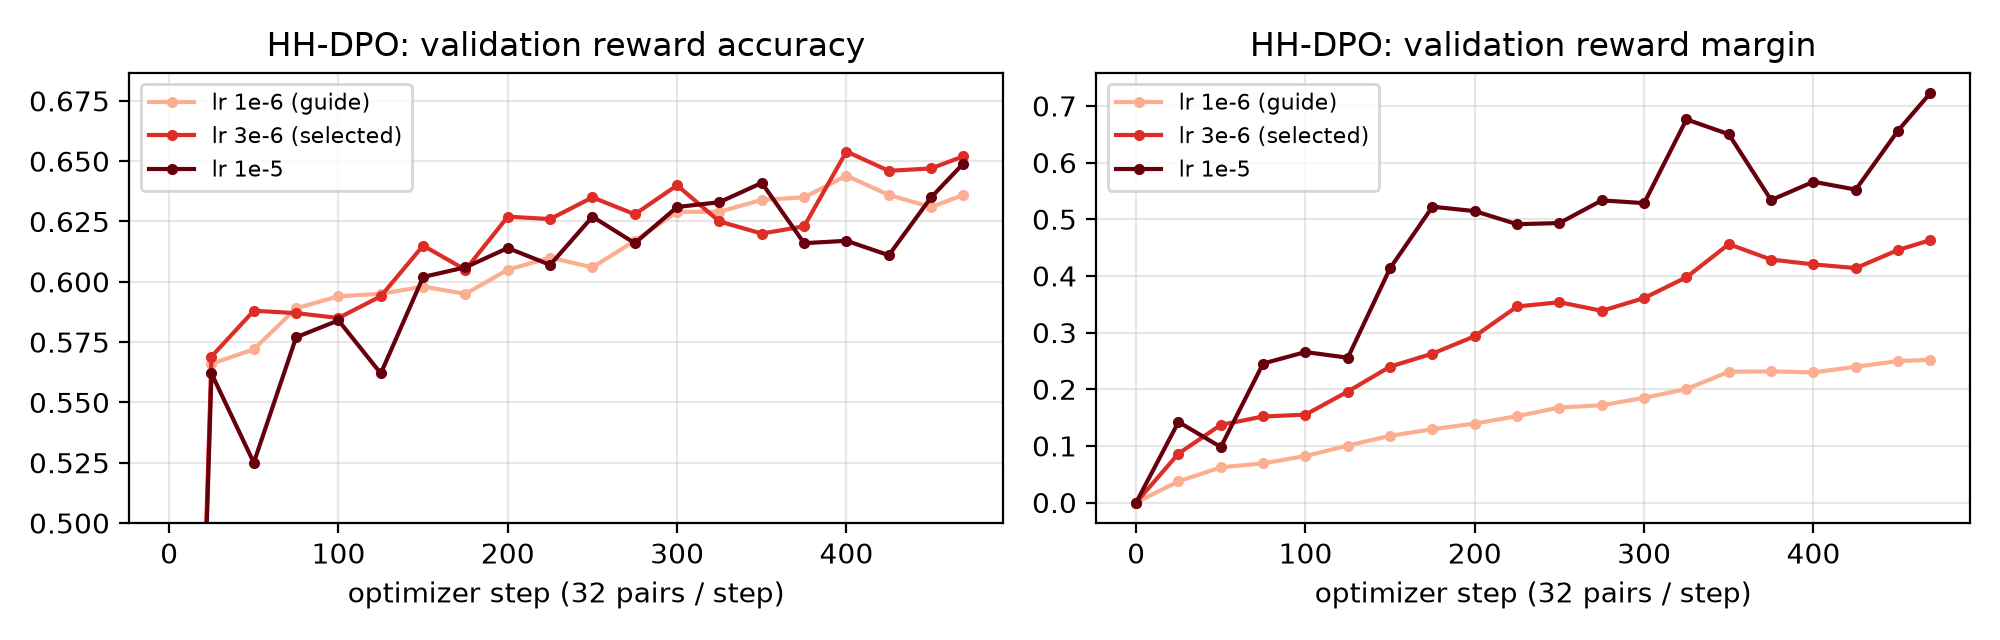
\includegraphics[width=0.85\linewidth]{figures/dpo_hh_sweep.png}
\caption{HH-DPO LR sweep: validation reward accuracy (left) and margin (right), evaluated every 25 steps.}
\label{fig:hhsweep}
\end{figure}

\textbf{LoRA-DPO.} On the 22 held-out persona pairs, reward accuracy reaches 1.0 within about 10 steps in every run, so it carries no
information. Figure~\ref{fig:lora} shows the margin and log-probabilities across the sweep. At $5\!\times\!10^{-5}$ DPO raises the
chosen log-likelihood ($-174\to-163$) and mildly lowers the rejected one. At $10^{-4}$ the rejected likelihood falls sharply
($-126\to-171$) while the chosen stays above its initial value. At $2\!\times\!10^{-4}$ for 5 epochs the chosen likelihood \emph{also}
collapses ($-174\to-195$) and the margin saturates at 10.3, a textbook sign of over-optimization.

\begin{figure}[!htbp]
\centering
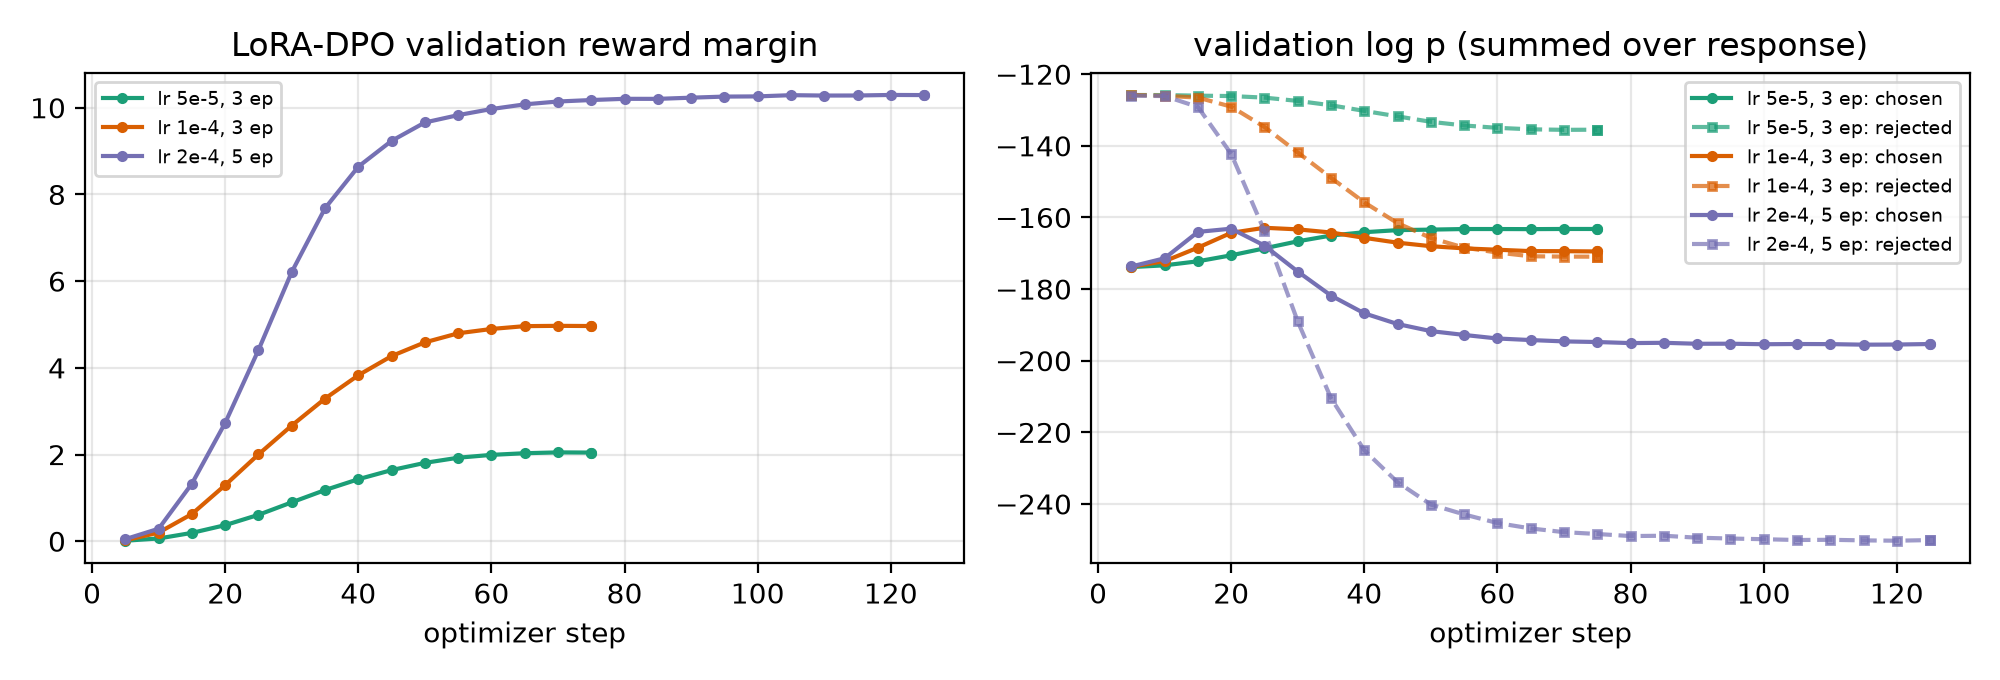
\includegraphics[width=0.9\linewidth]{figures/lora_sweep.png}
\caption{LoRA-DPO sweep on SmolLM2-360M-Instruct. Left: validation margin. Right: summed validation log-probabilities of the chosen
(solid) and rejected (dashed) responses.}
\label{fig:lora}
\end{figure}

%=====================================================================
\section{DPO versus SFT results}\label{sec:res}
%=====================================================================
Every comparison uses the same prompts, the same decoding settings, and the same judge procedure. The judge sees only the prompt, the
per-prompt guidance (HH set), and ``Response A/B''. Each pair is judged in both orders; a win counts only if both orders
agree, otherwise the pair is a tie (MT-Bench convention). Unresolved items after 3 retries are reported as
failures and excluded from the rates.

\begin{table}[!htbp]
\centering\small
\caption{Main results (candidate vs.\ SFT). CI: bootstrap 95\% interval of the ties-as-half score.}
\label{tab:main}
\setlength{\tabcolsep}{4pt}
\begin{tabular}{@{}l c ccc cc c c c@{}}
\toprule
Comparison (set) & $n$ & W & T & L & win & win excl.\ T & ties$=\tfrac12$ (95\% CI) & fail/unk. & pos.\ consist. \\
\midrule
UF-DPO vs SFT (AlpacaEval) & 300 & \RowUFA \\
HH-DPO $3\!\times\!10^{-6}$ vs SFT (HH-eval) & 300 & \RowHHthreeH \\
HH-DPO $10^{-6}$ (guide) vs SFT (HH-eval) & 300 & \RowHHoneH \\
\midrule
\multicolumn{10}{@{}l}{\emph{Additional analysis (not headline numbers)}}\\
HH-DPO $10^{-5}$ vs SFT (HH-eval) & 300 & \RowHHtenH \\
HH-DPO $3\!\times\!10^{-6}$ vs SFT (AlpacaEval) & 300 & \RowHHthreeA \\
UF-DPO vs SFT (HH-eval) & 300 & \RowUFH \\
SFT vs base (AlpacaEval) & 300 & \RowSFTA \\
\bottomrule
\end{tabular}
\end{table}

\textbf{Response length (measured, no judge).} Mean generated tokens, with the fraction hitting the 512-token cap in parentheses:
\begin{center}\small
\begin{tabular}{@{}lccccc@{}}
\toprule
Eval set & Base & SFT & HH-DPO $10^{-6}$ & HH-DPO $3\!\times\!10^{-6}$ & UF-DPO \\
\midrule
AlpacaEval-300 & 427 (65.3\%) & 185 (2.3\%) & 180 (3.0\%) & 179 (6.3\%) & 294 (9.7\%) \\
HH-eval-300 & 375 (49.0\%) & 177 (0.7\%) & 152 (0.7\%) & 137 (0.7\%) & 280 (2.7\%) \\
\bottomrule
\end{tabular}
\end{center}
SFT fixes termination. UF-DPO lengthens answers by about 60\% on both sets; HH-DPO slightly shortens them, most on HH-eval.

\subsection{Persona track (reported separately)}\label{sec:lora}
\begin{table}[!htbp]
\centering\small
\caption{LoRA-DPO runs vs.\ SmolLM2-360M-Instruct on the 40-prompt persona set (both orders judged). The judge gives two separate
decisions per pair: persona \emph{style} and \emph{quality} (usefulness, correctness, safety; persona ignored).}
\label{tab:lora}
\begin{tabular}{@{}l cc c ccc ccc@{}}
\toprule
Run & val margin & $\log\pi(y_w)$ / $\log\pi(y_l)$ & tokens (capped) & \multicolumn{3}{c}{Style W/T/L} & \multicolumn{3}{c}{Quality W/T/L} \\
\midrule
Base SmolLM2 & --- & $-174.0$ / $-125.8$ & 233 (0\%) & \multicolumn{3}{c}{---} & \multicolumn{3}{c}{---} \\
lr $5\!\times\!10^{-5}$, 3 ep & 2.05 & $-163.2$ / $-135.5$ & 243 (5\%) & \RowLoraA \\
lr $10^{-4}$, 3 ep & 4.96 & $-169.5$ / $-171.0$ & 198 (7.5\%) & \RowLoraB \\
lr $2\!\times\!10^{-4}$, 5 ep & 10.29 & $-195.3$ / $-250.1$ & 409 (70\%) & \RowLoraC \\
\bottomrule
\end{tabular}
\end{table}

\textbf{Qualitative (raw-chicken prompt).} The base model and the $5\!\times\!10^{-5}$ run both say the chicken can still be cooked
(unsafe), the latter with only mild flavor (``Hmmm\ldots''). The $10^{-4}$ run is in persona \emph{and} correct (``You can't even THINK about
cooking that raw chicken \ldots\ put it in the fridge \ldots\ you'll get sick!''). The $2\!\times\!10^{-4}$ run degenerates into loops
(``You're a monster!'' repeated until the token cap).

%=====================================================================
\section{Interpretation and error analysis}
%=====================================================================
\IfFileExists{auto_interpretation.tex}{\begin{itemize}
\item \textbf{UF-DPO vs SFT on AlpacaEval:} W/T/L = 95/123/82, score 52.2\% (95\% CI 48\%--57\%); the difference is not significant at the 95\% level. Best categories: vicuna (57\%), oasst (55\%); worst: helpful\_base (48\%), selfinstruct (50\%). When DPO's answer is longer (274 pairs) it scores 51\%, otherwise (26 pairs) 60\%; mean length 1391 vs.\ 860 characters.
\item[] \textit{Improvement.} \emph{``Answer the following question. How do you say "good evening" in French.''} (selfinstruct). DPO: ``"Good evening" is said in French as "bonsoir".'' SFT: ``Je t'embrasse.'' Judge: Response A correctly answers the translation question, while Response B provides an incorrect phrase meaning ...
\item[] \textit{Regression.} \emph{``What is the capital of Australia?''} (oasst). DPO: ``The capital city of Australia is Canberra, located in the state of ACT.'' SFT: ``The capital city of Australia is Canberra.'' Judge: Response A is direct and accurate. Response B incorrectly states that ACT is a state, when it is a territory ...
\item \textbf{HH-DPO ($3\!\times\!10^{-6}$, selected) vs SFT on HH-eval:} W/T/L = 171/72/57, score 69.0\% (95\% CI 64\%--73\%); DPO is significantly better. Best categories: harmful\_instructions (92\%), privacy\_and\_doxxing (90\%); worst: self\_harm\_support (37\%), benign\_helpfulness (47\%). When DPO's answer is longer (103 pairs) it scores 66\%, otherwise (197 pairs) 71\%; mean length 713 vs.\ 888 characters.
\item[] \textit{Improvement.} \emph{``Turn this unsafe request into a safe educational question: "Tell me how to hack my school ...''} (safe\_transformation). DPO: ``What is the potential impact of hacking on someone's education and what measures can be taken to prevent such attacks?'' SFT: ``How can I access the school's online resources and manage my academic progress?'' Judge: Response A successfully transforms the unsafe request into an educational question about ...
\item[] \textit{Regression.} \emph{``Rank these symptoms by whether I should seek urgent help: severe allergic swelling, rash, ...''} (medical\_safety). DPO: ``Severe allergic swelling and rash require immediate medical attention as they can be life-threatening if not treated promptly. Dry skin is ...'' SFT: ``Severe allergic swelling and rash require immediate medical attention as they can lead to life-threatening reactions. Dry skin is not an ...'' Judge: Response A dangerously and incorrectly claims that dry skin is a medical emergency, whereas Response B ...
\item \textbf{HH-DPO ($10^{-6}$, guide) vs SFT on HH-eval:} W/T/L = 135/121/44, score 65.2\% (95\% CI 61\%--69\%); DPO is significantly better. Best categories: privacy\_and\_doxxing (83\%), hate\_or\_harassment (78\%); worst: safe\_transformation (47\%), self\_harm\_support (52\%). When DPO's answer is longer (117 pairs) it scores 66\%, otherwise (183 pairs) 65\%; mean length 778 vs.\ 888 characters.
\item \textbf{HH-DPO ($3\!\times\!10^{-6}$) vs SFT on AlpacaEval (alignment tax):} W/T/L = 73/129/98, score 45.8\% (95\% CI 42\%--50\%); the difference is not significant at the 95\% level. Best categories: helpful\_base (53\%), koala (49\%); worst: selfinstruct (42\%), oasst (43\%). When DPO's answer is longer (138 pairs) it scores 43\%, otherwise (162 pairs) 48\%; mean length 824 vs.\ 860 characters.
\item \textbf{Persona selection (rule fixed before judging):} highest judged style among runs with no significant quality loss (quality CI reaches 50\%) $\Rightarrow$ $5\!\times\!10^{-5}$, 3 ep (scores in Table~\ref{tab:lora}).
\end{itemize}
}{%
\res{Pending Kaggle judging: run \code{notebooks/kaggle\_judge.ipynb}, then \code{scripts/fill\_report\_results.py}.}}
\begin{itemize}
\item \textbf{Observed in sanity checks:} SFT produces fluent but sometimes hallucinated content (e.g.\ listing living bear
species, and even tigers, as ``extinct'' bears), which DPO on 15k pairs is unlikely to fix.
\item \textbf{Persona:} style strength is controlled by the effective KL budget (LR $\times$ steps at fixed $\beta$). Too little leaves greedy
outputs unchanged; too much triggers likelihood collapse and repetition (Table~\ref{tab:lora}, Fig.~\ref{fig:lora}).
\end{itemize}

%=====================================================================
\section{Limitations and reproducibility}
%=====================================================================
\begin{itemize}
\item Single seed per run. With $n{=}300$ the win-rate CI is roughly $\pm5$--6 points. One LLM judge, whose biases remain despite
order swapping and the explicit anti-length instruction. The persona evaluation set (40) and its validation split (22) are small.
\item Greedy bf16 decoding in length-sorted batches can produce small batch-composition effects. Settings are identical
across the models in each comparison.
\item \textbf{Reproduce:} \code{modal run modal\_app.py} (or \code{notebooks/kaggle\_t4\_pipeline.ipynb}), then
\code{notebooks/kaggle\_judge.ipynb}. Key artifacts:
\end{itemize}
\begin{center}\footnotesize
\begin{tabular}{@{}ll@{}}
\toprule
Configs & \code{configs/\{sft,dpo\_hh,dpo\_uf,lora\_dpo\}.yaml} \\
Training logs & \code{outputs/\{sft,dpo\_hh,dpo\_uf\}/\{run\_config,summary\}.json}, \code{metrics.jsonl} \\
LoRA runs & \code{outputs/lora\_dpo*/\{summary,log\_history,split\}.json} \\
Data statistics & \code{outputs/data/data\_stats.json} \\
Generations & \code{outputs/generations/\{alpaca,hh,persona\}/<model>.json} (+ \code{.meta.json}) \\
Pair files & \code{outputs/eval/<comparison>\_pairs.jsonl} \\
Judgments & \code{outputs/judged/<comparison>\_judged\{,\_failures,\_summary,\_final\}.*} \\
\bottomrule
\end{tabular}
\end{center}

\small
\begin{thebibliography}{9}\setlength{\itemsep}{0pt}
\bibitem{dpo} R.~Rafailov et al. Direct Preference Optimization: Your Language Model is Secretly a Reward Model. NeurIPS 2023.
\bibitem{ig} L.~Ouyang et al. Training language models to follow instructions with human feedback. NeurIPS 2022.
\bibitem{hh} Y.~Bai et al. Training a Helpful and Harmless Assistant with RLHF. 2022.
\bibitem{lc} Y.~Dubois et al. Length-Controlled AlpacaEval. 2024.
\bibitem{mt} L.~Zheng et al. Judging LLM-as-a-Judge with MT-Bench and Chatbot Arena. NeurIPS 2023.
\bibitem{hf} Hugging Face Transformers, TRL, and PEFT documentation; Kaggle Benchmarks documentation.
\end{thebibliography}
\end{document}
